\chapter{Understanding a \uppaal model}\label{app:uppaal}
The goal of this appendix is not to give an extensive guide on how to use \uppaal, but rather to serve as a short introduction on how to read the models described in this report.
For a more in-depth description of how \uppaal works, we recommend the official tutorial for \uppaal 4.0 by Gerd Behrmann, Alexandre David and Kim G. Larsen \cite{uppaaltutorial}.

\section*{What is \uppaal?}
\uppaal is an integrated tool environment for modeling and verification of timed automata.
It is mainly used for simulating and verifying models of real-time systems \cite{uppaalintro} by means of property checking, where it can automatically generate a diagnostic trace to explain why a given property is, or is not, satisfied by the modeled system.\\
This property checking is done using a reachability analysis, meaning that it will search through the state space of the system to find a state where a given property is true.
Using property checking it is then possible to check for properties like whether or not the system can end up in a deadlock - or in the context of this system, it would be possible to check whether or not it is possible that one client is still in the lobby while the other clients are receiving in-game information such as positional data.

\section*{Format of a system in \uppaal}
A very basic model in \uppaal consists of a set of locations and edges as seen on \autoref{fig:app:uppaal:locations}.
In this basic model, we have two locations: \uppLoc{A} and \uppLoc{B} and two transitions: From \uppLoc{A} to \uppLoc{B}, and from \uppLoc{B} to \uppLoc{A}.
The location \uppLoc{A} has an extra ring, which indicates that it is an initial location, meaning that this is where the system will start when initialized.

\begin{figure}[H]
    \centering
    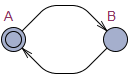
\includegraphics[]{uppaal/applocations.png}
    \caption{Locations in \uppaal.}
    \label{fig:app:uppaal:locations}
\end{figure}
\noindent
This visual model combined with a set of local declarations related to the model is called a template.

In addition to the local declarations, which are scoped to the current template, it is also possible to have global declarations (first object in the Project folder on \autoref{fig:app:uppaal:templates}), which are variables and functions that are shared across the entire system.

\begin{figure}[H]
    \centering
    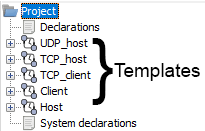
\includegraphics[]{uppaal/apptemplates.png}
    \caption{Content of a \uppaal project.}
    \label{fig:app:uppaal:templates}
\end{figure}
\noindent
When the system is started in the simulator, these \uppTemp{templates} will be instantiated as \uppProc{processes}, which start in their initial locations.

From here, the user can choose which transition to take next in the given process, as seen on Figures \ref{fig:app:uppaal:enabledtransitions} and \ref{fig:app:uppaal:transitions}.

\begin{figure}[H]
    \centering
    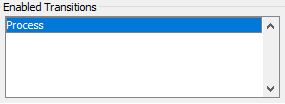
\includegraphics[]{uppaal/appenabledtransitions.png}
    \caption{Enabled traces of a process.}
    \label{fig:app:uppaal:enabledtransitions}
\end{figure}

\begin{figure}[H]
    \centering
    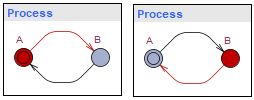
\includegraphics[]{uppaal/apptransitions.png}
    \caption{The process before and after taking the transition.}
    \label{fig:app:uppaal:transitions}
\end{figure}

\section*{Synchronizations}
As a \uppaal system can consist of multiple processes, it is often useful to allow the different processes to communicate.
One way of communicating is via the use of \uppSync{synchronizations}.
If a transition between two locations has a synchronization called sync on it, as seen in \autoref{fig:app:uppaal:sync}, it can wait for another process to communicate with it before taking the transition.

\begin{figure}[H]
    \centering
    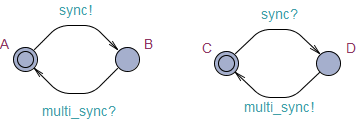
\includegraphics[]{uppaal/appsync.png}
    \caption{Model with synchronizations on transitions.}
    \label{fig:app:uppaal:sync}
\end{figure}
\noindent
In the model on \autoref{fig:app:uppaal:sync}, the \uppSync{sync} has an exclamation mark after its name, and on the other a question mark.
This means that A is the transmitter of a synchronization request and that it cannot take the transition before another process with a question mark (receiver) is ready to take a transition with a synchronization of the same name.
Likewise, it is not possible to take a transition with a \uppIn{sync} until another process is transmitting a \uppOut{sync}.
When this synchronization is ready to happen, both processes will take the transition.

In this basic example, it is easily seen that there is only one sender and one receiver for the synchronization.
In a larger example, there might be several processes ready to receive the synchronization, but only one can actually receive the transition at a time.

This is due to the implementation of synchronizations, where we synchronize using a channel defined in the global declarations:

\begin{uppaalcode}
chan sync;
\end{uppaalcode}
\noindent
However, should we want to synchronize with multiple other processes instead, it is possible to declare the synchronization channel as a broadcast channel instead:

\begin{uppaalcode}
broadcast chan multi_sync;
\end{uppaalcode}
\noindent
Having the channel defined as a broadcast means that any process that is ready to synchronize when a synchronization output is transmitted must do so.


\section*{Clocks, guards, and selections}
As mentioned previously, \uppaal works with timed automata - so let us add some time to our sample model.
To do this, we can add a \uppClock{clock} to the local declarations of our template using the clock type:
\begin{uppaalcode}
clock time;
\end{uppaalcode}
\noindent
We can now use this clock to, for example, limit which transitions can be taken from a given state using \uppGuard{guards}.

\begin{figure}[H]
    \centering
    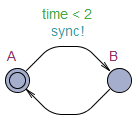
\includegraphics[]{uppaal/appguard.png}
    \caption{Model with a guard.}
    \label{fig:app:uppaal:guard}
\end{figure}
\noindent
In the example on \autoref{fig:app:uppaal:guard}, a \uppGuard{guard} has been added on the transition from \uppLoc{A} to \uppLoc{B}, specifying that at most two time units must have passed before this transition can be taken.

This quickly poses a problem for us, though, as the time will keep increasing, meaning that we may not be able to take the transition from \uppLoc{A} to \uppLoc{B} again, and will end up in a deadlock.

\begin{figure}[H]
    \centering
    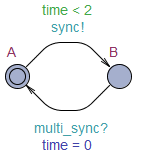
\includegraphics[]{uppaal/appselection.png}
    \caption{Model with a guard and selection.}
    \label{fig:app:uppaal:selection}
\end{figure}
\noindent
To fix this, it is possible to use updates to update the value of the clock, as seen in \autoref{fig:app:uppaal:selection} where we reset the \uppClock{time} to 0 when taking the transition from \uppLoc{B} to \uppLoc{A}.

\section*{Invariants}
Much like guards limit the possibility of taking a transition until some conditions have met, invariants can be used to limit when it is possible to be in a given location.
In \autoref{fig:app:uppaal:invariant} we have added an invariant to \uppLoc{B}, specifying that less than 8 \uppClock{time} units must have passed before it leaves the transition.

If the invariant conditions are not met, the process cannot enter the location or must leave it as soon as the conditions no longer hold.
\begin{figure}[H]
    \centering
    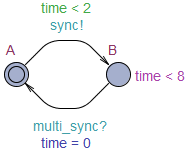
\includegraphics[]{uppaal/appinvariant.png}
    \caption{Model with an invariant on location B.}
    \label{fig:app:uppaal:invariant}
\end{figure}

\section*{Committed and urgent locations}
Urgent locations are locations where time is not able to pass.
This means that if any of the processes are currently in an urgent location, all clocks in the system are paused until the process transitions out of that location.
Just like in urgent locations, time cannot pass in committed locations.
In addition to this, if any process is in a committed location, the next transition that happens in the system has to be from a process that is in a committed location. 
The main difference between these two is that while a process is in an urgent location, other processes are still able to take transitions while if a process is in a committed location, the only processes that are able to take a transition are processes that are in a committed location.
Examples of how the syntax for these two looks can be seen on \autoref{fig:app:uppaal:committed}.

\begin{figure}[H]
    \centering
    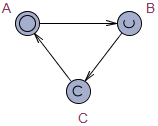
\includegraphics[]{uppaal/appcommittedurgent.png}
    \caption{Model with committed and urgent locations.}
    \label{fig:app:uppaal:committed}
\end{figure}
\noindent

Location \uppLoc{B} is an urgent location and location \uppLoc{C} is a committed location.

\section*{Verification}
In addition to being a modeling tool, UPPAAL has a built-in verifier which allows the user to check if a given condition can hold true in the system.
This allows for checking things like whether the system can end up in a deadlock or if a given state can ever be reached.
To formulate these queries, there are four key elements:\\
$E$ to check if there exists a path, meaning that it will return true if there is at least one trace through the system where the condition holds true.\\
$A$ to check if the condition holds true for all paths.\\
$[]$ to check if the condition holds for all states in the path.\\
$<>$ to check if the condition holds for at least one state in the path.\\
This results in four different kinds of queries: $E[]$, $A[]$, $E<>$ and $A<>$.\\\\

All of these possibilities are followed by a predicate, $p$ specifying exactly which property you are interested in checking for.
This means that the query $A<>p$ is read as "For all paths in the automaton, it is true that in at least one state p is satisfied."
